\documentclass[11pt,a4paper]{report}

\usepackage{amsmath}
\usepackage{amssymb}
\usepackage{graphicx}
\usepackage{float}
\usepackage{geometry}
\usepackage{hyperref}
\usepackage{booktabs}
\usepackage{listings}
\usepackage{xcolor}
\usepackage{tikz}
\usepackage{enumitem}
\usepackage{longtable}
\usepackage{subcaption}
\geometry{margin=1in}
\usepackage{newtxtext,newtxmath}
\title{Gait IK of quadruped robot}

\date{}

\begin{document}
\setcounter{tocdepth}{1}
\maketitle
\tableofcontents
%%%%%%%%%%%%%%%%%%%%%%%%%%%%%%%%%%%%%%%%%%%%%%%%%%%%%%%%%%%%%
\chapter{Trot motion}
\section{Locomotion Command Representation}

\subsection{Desired Body Motion}

The  controller is fundamentally a velocity-tracking
controller.The operator specifies a desired body motion represented by

\[
u=
\begin{bmatrix}
v_x\\
v_y\\
\dot{\psi}
\end{bmatrix}
\]

where

\begin{itemize}
\item $v_x$ is the desired forward velocity,
\item $v_y$ is the desired lateral velocity,
\item $\dot{\psi}$ is the desired yaw rate,
\end{itemize}


\section{Gait Scheduling}
\subsection{Contact Phase Matrix for trot motion }

\[
C=
\begin{array}{c|cccc}
&
\phi=\frac14 &
\phi=\frac12 &
\phi=\frac34 &
\phi=1
\\ \hline
FR & 1 & 1 & 1 & 0\\
FL & 1 & 0 & 1 & 1\\
RR & 1 & 1 & 1 & 0\\
RL & 1 & 0 & 1 & 1
\end{array}
\]
\subsection{Phase Timing}

Define:

\begin{itemize}
\item Stance Time
\item Swing Time
\end{itemize}

%%%%%%%%%%%%%%%%%%%%%%%%%%%%%%%%%%%%%%%%%%%%%%%%%%%%%%%%%%%%%
\section{Stance Controller Based on COM Motion}

\subsection{Commanded Body Motion}

The desired locomotion command is

\[
u=
\begin{bmatrix}
v_x\\
v_y\\
\omega
\end{bmatrix}
\]

where

\begin{itemize}
\item $v_x$ is the forward velocity,
\item $v_y$ is the lateral velocity,
\item $\omega$ is the body yaw rate.
\end{itemize}

During one stance interval of duration

\[
T_{stance}
\]

the desired body displacement is

\[
\Delta x_{COM}
=
v_x T_{stance}
\]

\[
\Delta y_{COM}
=
v_y T_{stance}
\]

and the desired body rotation is

\[
\theta
=
\omega T_{stance}.
\]

These quantities define the desired rigid-body motion of the robot during the stance phase.
\begin{figure}[htbp]
\centering

\begin{subfigure}{\linewidth}
    \centering
    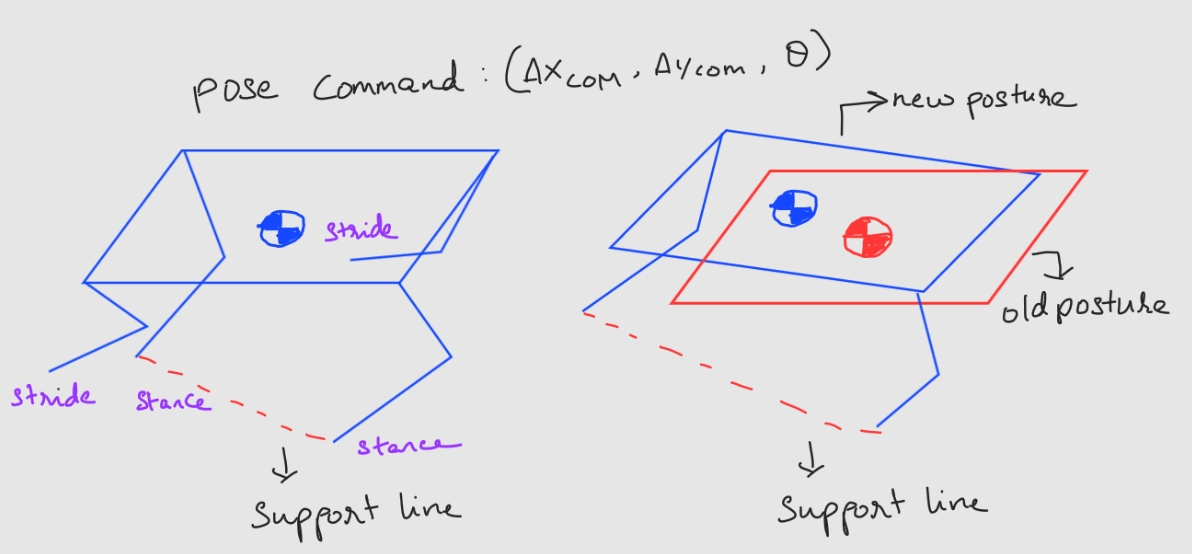
\includegraphics[width=0.5\linewidth]{trot_ik_imgs/stance_body.jpg}
    \caption{Body motion generated during stance.}
    \label{fig:stance_body}
\end{subfigure}

\vspace{0.5cm}

\begin{subfigure}{\linewidth}
    \centering
    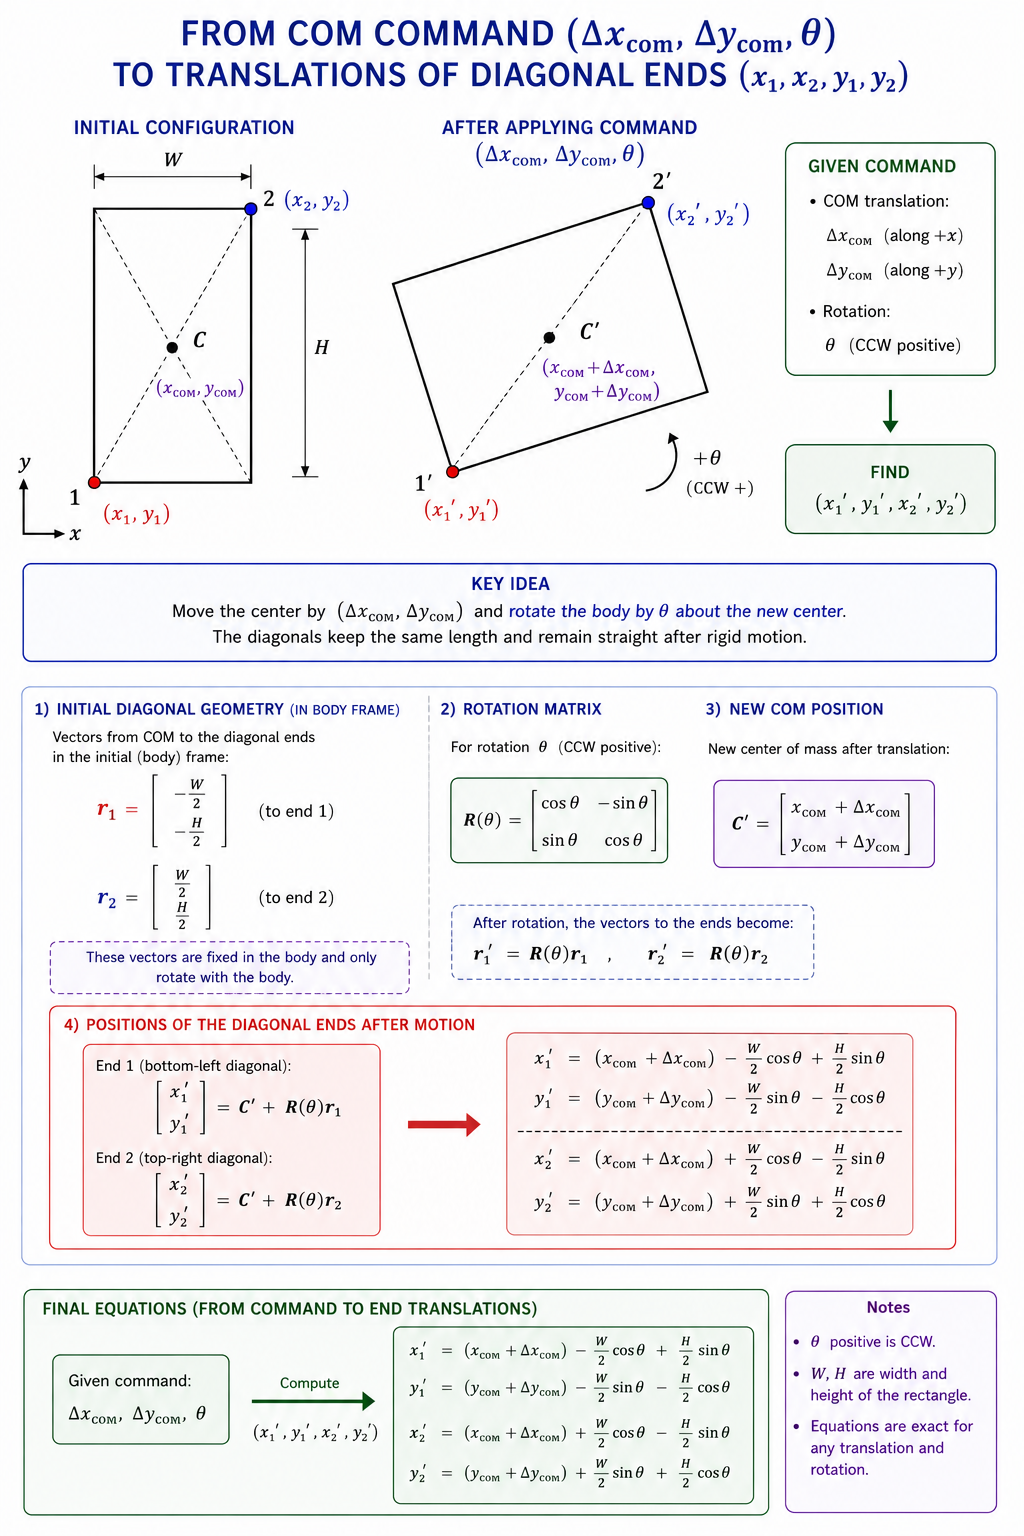
\includegraphics[width=0.9\linewidth]{trot_ik_imgs/stance_control.png}
    \caption{Corresponding hip displacement computation.}
    \label{fig:stance_control}
\end{subfigure}

\caption{COM-based stance controller.}
\label{fig:stance_combined}
\end{figure}

\subsection{Control Algorithm}

At every stance update:

\begin{enumerate}
\item Receive command

\[
(v_x,v_y,\omega)
\]

\item Compute the desired body motion during the stance interval

\[
\Delta x_{COM} = v_xT_{stance}
\]

\[
\Delta y_{COM}=v_yT_{stance}
\]

\[
\theta=\omega T_{stance}.
\]

\item Compute the required hip joint displacements for the two
diagonally opposite stance legs using the rigid-body equations shown in
Figure~\ref{fig:stance_control}.

\item Obtain

\[
(\Delta x_1,\Delta y_1,\Delta x_2,\Delta y_2).
\]

\item Compute the desired hip positions

\[
\mathbf{P}_{H_i}'
=
R(\theta)\,
\mathbf{P}_{H_i}
+
\begin{bmatrix}
\Delta x_{COM}\\
\Delta y_{COM}
\end{bmatrix}.
\]

\item Since the stance feet remain fixed on the terrain,

\[
\mathbf{P}_{F_i}'
=
\mathbf{P}_{F_i}.
\]

\item Compute the desired foot position relative to the new hip frame

\[
    \mathbf{P}_{F_iREL}
=
\mathbf{P}_{F_i}
-
\mathbf{P}_{H_i}'.
\]

This represents the location of the fixed foot with respect to the
desired hip position.

\item Use the standard 3-DOF leg inverse kinematics solver to compute
the required joint angles

\[
(q_{abd},q_{hip},q_{knee})
=
IK
\left(
{}^{H_i}\mathbf{p}_{F_i}
\right).
\]

\item Send the computed joint commands to the leg actuators.
\end{enumerate}
%%%%%%%%%%%%%%%%%%%%%%%%%%%%%%%%%%%%%%%%%%%%%%%%%%%%%%%%%%%%%

\section{Swing Phase Controller}

\subsection{Role of the Swing Phase}

During the swing phase, the foot is no longer in contact with the
terrain and therefore cannot contribute to support or propulsion.

The objective of the swing controller is to reposition the swing foot
such that an appropriate support polygon is established for the next
stance phase.

Since the stance controller generates body motion through the commanded

\[
(\Delta x_{COM},\Delta y_{COM},\theta),
\]

the swing controller must place the foot so that the next support
configuration is compatible with this new body pose.

\subsection{Touchdown Location Generation}

Let

\[
p_{nom}
\]

denote the nominal touchdown location of a swing foot expressed in the
body frame.

For example,

\[
p_{FR,nom}
=
\begin{bmatrix}
\frac{L}{2}\\
-\frac{W}{2}\\
-h
\end{bmatrix}
\]

for the front-right leg and

\[
p_{RL,nom}
=
\begin{bmatrix}
-\frac{L}{2}\\
\frac{W}{2}\\
-h
\end{bmatrix}
\]

for the rear-left leg.

These nominal positions define the desired support geometry of the
quadruped when standing.

During the stance phase, the body undergoes the commanded rigid-body
motion

\[
(\Delta x_{COM},\Delta y_{COM},\theta).
\]

Since the stance feet remain fixed on the terrain, their coordinates
expressed in the body frame change according to the inverse body motion

\[
p_{stance,new}
=
R_z(-\theta)
\left(
p_{stance,old}
-
\begin{bmatrix}
\Delta x_{COM}\\
\Delta y_{COM}\\
0
\end{bmatrix}
\right).
\]

Thus, from the perspective of the moving body, the stance feet appear
to move backward.

To restore the nominal support geometry at the next touchdown event,
the swing foot must be placed ahead by the same amount.

The desired touchdown position is therefore obtained by applying the predicted body motion to the nominal foot location. To ensure stability and counteract drift, a Raibert-style heuristic is employed. Instead of just considering the past stance displacement, the predicted body travel over a future time horizon $T_{horizon}$ is used:
\[
T_{horizon} = \frac{T_{stance}}{k} + T_{swing}
\]
where $k$ is a tuning divisor (e.g., $1.2$ for the trot). 

\textbf{Note on the Raibert Heuristic:} Why use this formulation instead of just placing the foot where the body will be at the end of $T_{swing}$? If the foot is placed directly under the hip at touchdown, the body's forward motion during the stance phase will immediately cause the leg to trail behind the robot, creating an asymmetrical stance that pulls the robot backward. By adding a fraction of the stance time (e.g., $T_{stance}/2$), the heuristic commands the foot to land \textit{ahead} of the hip. This symmetrical motion balances the forces and keeps the Center of Mass stable.

The expected displacement for foot placement is:
\[
\Delta x_{TD} = v_x T_{horizon}, \quad \Delta y_{TD} = v_y T_{horizon}, \quad \Delta \theta_{TD} = \omega T_{horizon}
\]

The touchdown target becomes:
\[
p_{TD}
=
R_z(\Delta \theta_{TD})p_{nom}
+
\begin{bmatrix}
\Delta x_{TD}\\
\Delta y_{TD}\\
0
\end{bmatrix}.
\]
\\
$P_{TD}$ = touchdown location.\\
This placement ensures that after touchdown the new support pair
occupies the same relative configuration with respect to the body as
the previous stance pair occupied before the body motion occurred.

Consequently, the swing foot advances by exactly the amount that the
body moved relative to the fixed stance feet during the preceding
stance phase.\\
Use a smooth transition from $P_{nom}$ to $P_{TD}$ for natural motion.

%%%%%%%%%%%%%%%%%%%%%%%%%%%%%%%%%%%%%%%%%%%%%%%%%%%%%%%%%%%%%

\section{Inverse Kinematics}

\subsection{Closed-Form Inverse Kinematics Solution}

The hip abduction/adduction angle is

\[
\theta_1
=
\tan^{-1}\!\left(\frac{y}{x}\right)
+
\tan^{-1}
\!\left(
\frac
{\sqrt{x^2+y^2-l_2^2}}
{\pm l_2}
\right)
\]

where the sign depends on whether the leg belongs to the left or right
side of the robot.

The knee angle is

\[
\theta_3
=
-\cos^{-1}
\left(
\frac
{
\left(
\sqrt{
\left(
\sqrt{x^2+y^2-l_2^2}
-l_1
\right)^2
+z^2
}
\right)^2
-l_3^2-l_4^2
}
{2l_3l_4}
\right)
\]

The hip flexion/extension angle is

\[
\theta_2
=
\tan^{-1}
\left(
\frac
{z}
{\sqrt{x^2+y^2-l_2^2}-l_1}
\right)
-
\tan^{-1}
\left(
\frac
{l_4\sin(\theta_3)}
{l_3+l_4\cos(\theta_3)}
\right)
\]

Thus, the complete inverse kinematics solution becomes

\[
q=
\begin{bmatrix}
\theta_1\\
\theta_2\\
\theta_3
\end{bmatrix}.
\]

\subsection{Auxiliary Variables}

For compactness, the following auxiliary variables are introduced:

\[
F
=
\sqrt{x^2+y^2-l_2^2}
\]

\[
G
=
F-l_1
\]

\[
H
=
\sqrt{G^2+z^2}
\]

\[
D
=
\frac
{H^2-l_3^2-l_4^2}
{2l_3l_4}
\]

Using these definitions, the inverse kinematics equations can be written
more compactly as

\[
\theta_1
=
\tan^{-1}\!\left(\frac{y}{x}\right)
+
\tan^{-1}\!\left(\frac{F}{\pm l_2}\right)
\]

\[
\theta_3
=
-\cos^{-1}(D)
\]

\[
\theta_2
=
\tan^{-1}\!\left(\frac{z}{G}\right)
-
\tan^{-1}
\!\left(
\frac
{l_4\sin(\theta_3)}
{l_3+l_4\cos(\theta_3)}
\right)
\]
%%%%%%%%%%%%%%%%%%%%%%%%%%%%%%%%%%%%%%%%%%%%%%%%%%%%%%%%%%%%%
\chapter{Walking Mode}

\section{Overview of the Crawl Gait}

The walking mode is formulated as a quasi-static crawl gait. The objective is to move the quadruped forward while maintaining a sufficiently large support polygon for most of the gait cycle. In practice, this is achieved by ensuring that three or more feet remain in contact with the ground during stance-dominant portions of the cycle.

Unlike the trot gait, which uses diagonal pairing and more dynamic body motion, the crawl gait prioritizes stability over speed. The body advances slowly, and each swing leg is repositioned so that the next support configuration remains consistent with the commanded locomotion direction.

\section{Gait Scheduling and Phase Timing}

Let the normalized global gait phase be denoted by \(\phi_{global} \in [0,1)\). Each leg \(i\) is assigned a phase offset \(\phi_{offset,i}\), and its local phase is defined as
\[
\phi_i = (\phi_{global} + \phi_{offset,i}) \bmod 1.
\]

The crawl sequence is defined as
\[
RR \rightarrow FR \rightarrow RL \rightarrow FL.
\]

The phase offsets are chosen as
\[
\phi_{offset,FL}=0.00,\quad
\phi_{offset,RL}=0.25,\quad
\phi_{offset,FR}=0.50,\quad
\phi_{offset,RR}=0.75.
\]

A leg is in stance when
\[
\phi_i < d,
\]
and in swing when
\[
\phi_i \ge d,
\]
where \(d \in (0,1)\) is the duty factor. For a stable crawl gait, the duty factor is typically high, meaning that the stance phase occupies most of the cycle.

The stance duration and swing duration are
\[
T_{stance} = dT, \qquad T_{swing} = (1-d)T,
\]
where \(T\) is the total gait period.

\section{Stability Through Lateral Weight Shift}

During single-leg swing, the robot shifts its body laterally toward the stance side to improve the support margin. This shift is not the source of forward locomotion; rather, it is a stability mechanism that helps keep the projected center of mass inside the support polygon.

Let \(y_{shift}\) denote the desired lateral displacement of the trunk relative to the nominal body frame. A simple two-mode policy is
\[
y_{target} =
\begin{cases}
+Y_{max}, & \text{when the right-side legs are swinging},\\
-Y_{max}, & \text{when the left-side legs are swinging}.
\end{cases}
\]

To avoid discontinuities in the inverse kinematics, the lateral shift is smoothed over time:
\[
y_{shift,k} = y_{shift,k-1} + \alpha (y_{target} - y_{shift,k-1}),
\]
with
\[
\alpha = \min\!\left(1, \frac{\Delta t}{t_{ramp}}\right).
\]

Here \(t_{ramp}\) is a small blending time chosen so that the CoM shift evolves gradually during gait transitions.

\section{Stance Phase Motion}

During stance, the feet on the ground are treated as fixed contact points in the world frame. As the body advances, the foot positions relative to the body frame change, even though the feet themselves remain stationary on the terrain.

Let \(\mathbf{p}_{H_i}\) denote the hip position of leg \(i\), and let \(\mathbf{p}_{F_i}\) denote the stance foot position. If the body undergoes a desired displacement
\[
\Delta \mathbf{p}_{COM} =
\begin{bmatrix}
\Delta x_{COM}\\
\Delta y_{COM}
\end{bmatrix}
=
\begin{bmatrix}
v_x T_{stance}\\
v_y T_{stance}
\end{bmatrix},
\]
and a yaw change
\[
\Delta \psi = \omega T_{stance},
\]
then the desired hip position after the stance motion can be written as
\[
\mathbf{p}_{H_i}' = R_z(\Delta \psi)\mathbf{p}_{H_i} + \Delta \mathbf{p}_{COM}.
\]

Because the stance foot is assumed fixed on the ground,
\[
\mathbf{p}_{F_i}' = \mathbf{p}_{F_i}.
\]

Therefore, the stance foot expressed in the new hip frame is
\[
{}^{H_i}\mathbf{p}_{F_i}' = \mathbf{p}_{F_i}' - \mathbf{p}_{H_i}'.
\]

This relative position is then passed to the inverse kinematics solver to obtain the joint angles required to maintain stance while the body moves forward.

\section{Swing Phase Motion}

When a leg enters swing, it is no longer supporting the body and must be repositioned for the next touchdown. The swing trajectory is designed to satisfy two requirements:
\begin{enumerate}
    \item the foot must move smoothly from lift-off to touchdown,
    \item the foot must clear the ground during the swing phase.
\end{enumerate}

Let \(\mathbf{p}_{start}\) denote the foot position at lift-off and \(\mathbf{p}_{TD}\) the desired touchdown location. A normalized swing progress variable \(s \in [0,1]\) is defined by
\[
s = \frac{\phi_i - d}{1-d}.
\]

A smooth interpolation function may be used for the horizontal motion:
\[
s_{smooth} = s^2(3-2s).
\]

The horizontal swing path is then
\[
\mathbf{p}_{xy}(s) = (1-s_{smooth})\mathbf{p}_{start,xy} + s_{smooth}\mathbf{p}_{TD,xy}.
\]

The vertical trajectory is chosen to provide sufficient ground clearance:
\[
z(s) = (1-s_{smooth})z_{start} + s_{smooth}z_{TD} + h_{step} \, 4s(1-s),
\]
where \(h_{step}\) is the swing clearance height.

This trajectory produces a smooth liftoff, a clear mid-swing apex, and a gentle touchdown.

\section{Touchdown Placement}

The touchdown location is chosen so that the support geometry after landing is compatible with the commanded body motion. A simple heuristic is to place the next foothold ahead of the current support location by an amount proportional to the motion expected during the stance interval.

For a commanded body velocity
\[
u =
\begin{bmatrix}
v_x\\
v_y\\
\omega
\end{bmatrix},
\]
the nominal body displacement is calculated using a Raibert-style heuristic that considers the necessary forward placement to maintain balance over the swing phase:
\[
T_{horizon} = \frac{T_{stance}}{k} + T_{swing}
\]
where $k$ is a tuning divisor (e.g., $0.7$ for the static walk) used to ensure sufficiently aggressive foot placement and counteract backward drift in open-loop execution. The predicted displacement is:
\[
\Delta x = v_x T_{horizon}, \qquad
\Delta y = v_y T_{horizon}, \qquad
\Delta \psi = \omega T_{horizon}.
\]

If \(\mathbf{p}_{nom}\) denotes the nominal foothold position in the body frame, then the touchdown target is
\[
\mathbf{p}_{TD,xy} = R_z(\Delta \psi)\mathbf{p}_{nom,xy}
+ \begin{bmatrix}
\Delta x\\
\Delta y
\end{bmatrix}.
\]

This ensures that the faster the robot is commanded to move, the farther the swing foot must land ahead to prevent the body from lagging behind the support pattern.

\chapter{Additional Gaits}
The quadruped controller framework has been extended to support several other gaits by modifying the gait parameters and phase offsets. 

\section{Walking Trot and Flying Trot}
The trot gait is characterized by diagonal legs moving in sync ($\phi_{FR}=\phi_{RL}=0.0$, $\phi_{FL}=\phi_{RR}=0.5$). Depending on the duty factor and period, different variations of the trot emerge:
\begin{itemize}
    \item \textbf{Walking Trot:} $T = 0.5$ s, $d = 0.6$. The duty factor $> 0.5$ ensures that there is always at least two legs on the ground, and for brief periods, all four legs may be in contact.
    \item \textbf{Trot:} $T = 0.4$ s, $d = 0.5$. The standard trot with exactly two legs in contact at any time.
    \item \textbf{Flying Trot:} $T = 0.3$ s, $d = 0.4$. The duty factor $< 0.5$ creates an aerial phase where all four legs are off the ground, suitable for higher speeds.
\end{itemize}

\section{Pacing Gait}
In the pacing gait, the lateral legs move in sync (the right legs together, and the left legs together). 
\begin{itemize}
    \item \textbf{Phase Offsets:} $\phi_{FR}=\phi_{RR}=0.0$, $\phi_{FL}=\phi_{RL}=0.5$.
    \item \textbf{Typical Parameters:} $T = 1.0$ s, $d = 0.8$. (Can be adjusted for faster pacing).
\end{itemize}

\section{Bounding Gait}
In the bounding gait, the front legs move together, and the rear legs move together.
\begin{itemize}
    \item \textbf{Phase Offsets:} $\phi_{FR}=\phi_{FL}=0.0$, $\phi_{RR}=\phi_{RL}=0.5$.
    \item \textbf{Typical Parameters:} $T = 0.4$ s, $d = 0.5$.
\end{itemize}

\section{Pronking Gait}
In the pronking gait, all four legs move in unison.
\begin{itemize}
    \item \textbf{Phase Offsets:} $\phi_{FR}=\phi_{FL}=\phi_{RR}=\phi_{RL}=0.0$.
    \item \textbf{Typical Parameters:} $T = 0.4$ s, $d = 0.5$.
\end{itemize}


\end{document}